\section{Background and Related Work}\label{sec:Related}

This section delves into the background needed to understand the presented research and compare it with prior efforts.

\subsection{Background on Offline Reinforcement Learning}
% Unlike the supervised machine learning algorithm, RL algorithm do not depend on the true value for training. An RL agent, during the training phase, constantly interacts with the system to evaluate the policy generated by the policy neural network or otherwise the actor network and train itself using the reward returned by the environment or the system. This method is hence called online RL and is not suitable for real-world settings such as autonomous driving, robot control, plat operations etc. where random actions cannot be applied to the system on account of plant security or cost involved. Therefore the offline RL aims to use the prior collected data from experimentation or random human demonstrations to learn the behavior and thereby reduce/ remove the interactions with the system. 

% Unlike supervised machine learning algorithms, RL algorithms do not depend on labeled data for training. Instead, an RL agent interacts with the system, evaluates the policy by testing the actions directly on the system, and trains by using the reward returned by the environment. 
% RL is represented by using a Markov decision process, $\mathcal{M} := (\mathcal{S},\mathcal{A}, \mathcal{R}, \mathbf{T}, \gamma)$, where $\mathcal{S}$ is the set of states that are observable information of the environment; $\mathcal{A}$ is the action space; $\mathcal{R}$ is the reward function, which is a mapping from $(\mathcal{S} \times \mathcal{A} \times \mathcal{S}) \rightarrow \mathbb{R}$; $\mathbf{T}$ is the transition probability function, $\mathcal{S} \times \mathcal{A} \rightarrow \mathcal{S}$, following which the transition from the present state $s(t)$ to the next state $s(t+1)$ occurs under the action $a(t)$ while obtaining the reward $r(s,a)$; and $\gamma \in [0,1]$ is the discount factor, which determines how much importance the agent has to give to the long-term rewards rather than the immediate rewards.   The goal of any RL agent is to find a policy $\pi$, which is a mapping from each state in $\mathcal{S}$ to $\mathcal{A}$, that maximizes the total sum of discounted rewards (called the return or the $Q$ value) along the trajectory of experience. 

% This online RL approach can be unsuitable, however, for certain real-world applications such as autonomous driving or robot control, where random actions cannot be applied to a live system because of safety or cost concerns. In the HPC domain, training an RL agent online can induce both computational and communication overhead due to the competition between the training algorithm and run time application for resources. This makes the data corrupted and unsuitable for learning. Another possibility is to separate the training node from the application node, which introduces the challenges of latency between observation and control. Therefore, in this paper we use offline RL~\cite{levine2020offline} to learn a policy from a static, pre-collected dataset that are easily available for HPC scientists. 
% This dataset, which is considerably smaller than the full action-state domain under consideration, is gathered by using arbitrary policies. The offline training
Reinforcement learning (RL) formulates control as a sequential decision-making problem, typically modeled as a Markov decision process (MDP) $\mathcal{M} := (\mathcal{S}, \mathcal{A}, \mathcal{R}, \mathbf{T}, \gamma)$, where an agent observes the system state $s \in \mathcal{S}$, selects an action $a \in \mathcal{A}$, and receives a reward $r \in \mathcal{R}$. The objective is to learn a policy $\pi : \mathcal{S} \rightarrow \mathcal{A}$ that maximizes the expected discounted return.
% The algorithm then uses this dataset to learn an optimal policy without further system interactions. We note that no mainstream RL algorithm, including Conservative Q-learning (CQL) \cite{levine2020offline}, is capable of taking actions it has never seen during training. Therefore, we ensure that the dataset exhaustively samples the action space at least once across different applications and hardware combinations. 

\iffalse 
% Akhilesh, we have already said that online RL is not acceptable for us. Let us skip this to save space
% Akhilesh, above is an older comment but still valid.
While RL is commonly trained through online interaction with the environment, such an approach is often impractical in real-world systems. In HPC settings, online training can interfere with application execution, introduce measurement noise, and incur unacceptable computational overhead. To avoid these issues, we adopt offline RL~\cite{levine2020offline}, which learns control policies from static, pre-collected datasets without requiring interaction with the live system during training.
\fi 

% In an offline RL setting such as the Q-learning we use in this paper, we cannot evaluate an unaccounted state-action pair during the training phase. Instead, we rely on the ability of the Q-network to learn from the available dataset a value function, given any state. A common challenge associated with using such an offline dataset for training an RL agent is distributional shift. This refers to a situation where the distribution of states and actions being encountered during training differs from the real-world behavior, thereby adversely impacting the trained agent performance. Another challenge associated with offline RL is its suboptimal performance when trained using a random policy.
% Here we use CQL \cite{levine2020offline} for training the RL-agent, a version of offline RL that regularizes the policy to avoid overestimation of the Q-values. By carefully choosing the learning parameters, we train an offline CQL agent from a previously collected dataset without overfitting. However, the knowledge of the system to be controlled can help populate the dataset with greedy policies to ensure near optimal behavior of the controller.
% We recall here the mathematical form of the loss function of CQL below for the reader’s understanding.

In an offline RL setting, such as the Q-learning approach used in this paper, unobserved state–action pairs cannot be evaluated during training. Instead, learning relies on the ability of the Q-network to approximate a value function from the available dataset. A common challenge in this setting is distributional shift, which arises when the distribution of states and actions encountered during training differs from that observed at deployment, potentially degrading performance. Another limitation of offline RL is suboptimal learning when trained solely from random policies.

To address these challenges, we employ Conservative Q-Learning (CQL)~\cite{levine2020offline}, which regularizes Q-value estimation to mitigate overestimation under distributional shift. By carefully selecting learning parameters, we train an offline CQL agent from a previously collected dataset without overfitting. Moreover, incorporating domain knowledge of the controlled system enables the dataset to be populated with informative (greedy) behaviors, improving the quality of the learned policy. 

% Akhilesh, the following though nice, probably is not needed to understand anything that comes next
% So, to save space, I am commenting it out. I think later on just saying "reduce the CQL loss func" 
% should be fine.
\iffalse 
We recall the mathematical form of the CQL loss function below for completeness.


%\vspace{-0.5cm}
% \begin{equation}
% \begin{aligned}
%     \min_Q \overbrace{\max_{\mu} \Big(\mathbb{E}_{s\sim \mathcal{D}}\mathbb{E}_{a(t) \sim \mu(a(t) \vert s(t))}[Q(s(t),a(t))]} ^{\text{Minimize the big Q-values}}- \overbrace{\mathbb{E}_{s(t),a(t) \sim \mathcal{D}}[Q(s(t),a(t))]\Big)}^{\text{Maximize the data Q-values}} \\ + \underbrace{\frac{1}{2\alpha}\mathbb{E}_{s(t),a(t),s(t+1) \sim \mathcal{D}}[(Q(s(t),a(t))-r(s(t),a(t)) - \gamma \mathbb{E}_{a(t+1) \sim \pi_{\theta}(a(t+1)\vert s(t+1))[Q(s(t+1),a(t+1))]})^2]}_{\text{Standard TD error}} 
% \end{aligned}
% \label{eq:CQL}
% \end{equation}
% \vspace{-0.4cm}
\begin{equation}
% \vspace{-0.2cm}
\small
\begin{aligned}
    \min_Q \ & \overbrace{\max_{\mu} \Big(\mathbb{E}_{s\sim \mathcal{D}}\mathbb{E}_{a_t \sim \mu(a_t \vert s_t)}[Q(s_t,a_t)] - \mathbb{E}_{s_t,a_t \sim \mathcal{D}}[Q(s_t,a_t)]\Big)}^{\text{Conservative term}} \\
    & + \frac{1}{2\alpha}\mathbb{E}_{s_t,a_t,s_{t+1} \sim \mathcal{D}}[(Q(s_t,a_t) - r(s_t,a_t) \\& - \gamma \mathbb{E}_{a_{t+1} \sim \pi_{\theta}(a_{t+1} \vert s_{t+1})}[Q(s_{t+1},a_{t+1})])^2],
\end{aligned}
\label{eq:CQL}
% \vspace{-0.1cm}
\end{equation}
where $s_t,a_t$ represent, respectively, the present state and  action, $\mathbb{E}$ is the notation for expected value, $\mu$ is the current policy from which the action $a_t$ is chosen (initialized as random policy), $\mathcal{D}$ is the state distribution under policy $\mu$, $\alpha$ is the conservative learning factor that determines how the RL agent reacts to out of distribution data, and $\pi_{\theta}$ represents the parameterized target policy, where $\theta$ represents the weights of the Q-network.
\fi 
% In Equation~\ref{eq:CQL}, the first part (regularization) minimizes distributional shift while second part minimizes the Bellman error.
 
% \subsection{Reward Function}
% Initially, we used a straightforward reward function that simply inverts the power consumption within each scheduling window: $R1(s, a) = -power$, where $s$ represents the progress value and $a$ the PCAP taken. While this function favors configurations with lower power usage, it does not account for performance impacts.

% To more effectively balance energy conservation with performance, we examine a metric that measures the performance divided by power. This can be seen as a variation of the energy-delay product (EDP), where delay is interpreted as the average time per instruction. Given our focus on HPC workloads, it's important to heavily penalize increased delays, which prompts us to consider a third potential reward function: $(progress)^3/PCAP$, resembling an inverse of $(EDP)^2$ on an instruction basis. To ensure a consistent increase in rewards, we scale $(progress)^2/PCAP$ and $(progress)^3/PCAP$ by a fixed constant $c$ where $(c >= 10)$, yielding two new reward function alternatives $R2(s, a) =  \times (progress)^2/W$ and $R3(s, a) = c \times (progress)^3/W$.

% In Section 5.6, we validate empirically that our preferred reward function R3(s, a) = (c×IPC)^3/W, drives the strongest overall performance, making it the chosen reward function for our system.
% \begin{algorithm}
%     \SetAlgoLined
%     \KwIn{Finite Dataset $\mathcal{D}$, Learning Rate $\alpha$, Discount factor $\gamma$}
%     \KwData{Critic Net $Q_\phi$}
%     \KwIn{Replay Buffer of size $b$ with transitions and rewards $\mathcal{B} \leftarrow \{(s_i, a_i, r_i, s_i')\}$}
%     \For{$\text{training iteration } t \in \{0, \dots, T\}$}{
%         \For{$i \leftarrow 0$ \KwTo $b$}{
%             Sample $(s_i, a_i, r_i, s_i')$ uniformly from $\mathcal{D}$\;
%         }
%         % $\tilde{s}_j \leftarrow g_\psi(s_j)$\;
%         $L_{\text{critic}} \leftarrow \frac{1}{B} \sum_{i=0}^{B} \left( Q_\phi({s}_i', a_i) - \mathbb{E}_{a' \sim \pi_\theta({s}_i')} \left[ (r_i + \nabla\gamma(Q_\phi({s}_i, a')))^2 \right] \right)$\;
%         % $\hat{A}(\tilde{s}_i, a_i) \leftarrow Q_\phi(\tilde{s}_i, a_i) - \frac{1}{k} \sum_{j=0}^{k} Q_\phi(\tilde{s}_i, a_j' \sim \pi_\theta(\tilde{s}_i))$\;
%         % $L_{\text{actor}} \leftarrow \frac{1}{B} \sum_{i=0}^{B} \left( -1_{\{ \hat{A}(\tilde{s}_i, a_i) > 0 \}} \log \pi_\theta(a_i | \tilde{s}_i) \right)$\;
%         % $\psi \leftarrow \psi - \alpha \nabla_\psi L_{\text{critic}}$\;
%         $\phi \leftarrow \phi - \alpha \nabla_\phi L_{\text{critic}}$\;
%         % $\theta \leftarrow \theta - \alpha \nabla_\theta L_{\text{actor}}$\;
%     }
%     \KwOut{Trained Scheduling Policy $argmax(Q_\phi(s))$}
%     \caption{Offline Training Algorithm}
% \end{algorithm}

% \begin{figure*}[htb]
%     \centering
%     \begin{subfigure}[b]{0.5\textwidth}
%         \centering
%         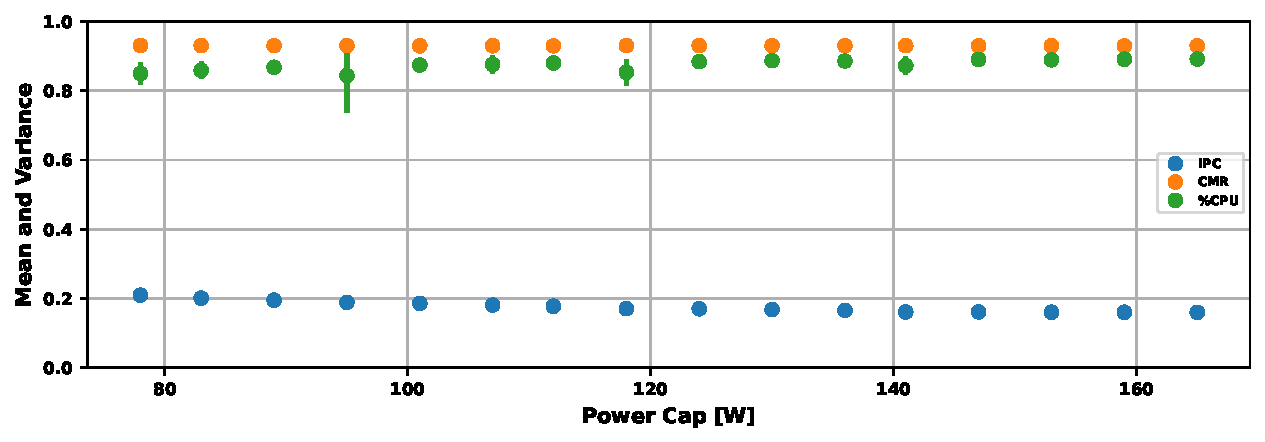
\includegraphics[width=\textwidth]{Figures/PAPI_stats_ones-stream-full.pdf}
%         % \caption{$Stream-Full$}
%         \label{fig:stream_perf}
%     \end{subfigure}\hfill
%     \begin{subfigure}[b]{0.5\textwidth}
%         \centering
%         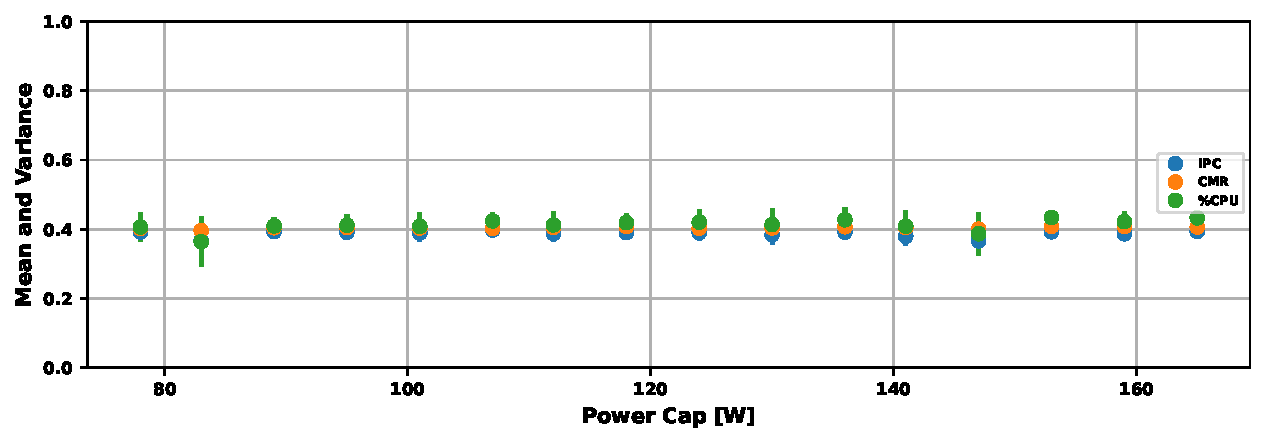
\includegraphics[width=\textwidth]{Figures/PAPI_stats_ones-npb-ep.pdf}
%         % \caption{$NPB-EP$}
%         \label{fig:ep_perf}
%     \end{subfigure}
%     \vspace{-1cm}
%     \caption{Average ($\mu$) and Standard deviation ($\sigma$) of IPC, CPU and CMR at various power levels for two of our benchmarks (Stream-full and NPB-EP). The experiments were repeated 10 times for each of the power caps.}
%     \label{fig:mu_sigma}
% %    \Description{Motivating example}
% \end{figure*}

% \begin{figure*}[htb]
%     \centering
%     \begin{subfigure}[b]{0.5\textwidth}
%         \centering
%         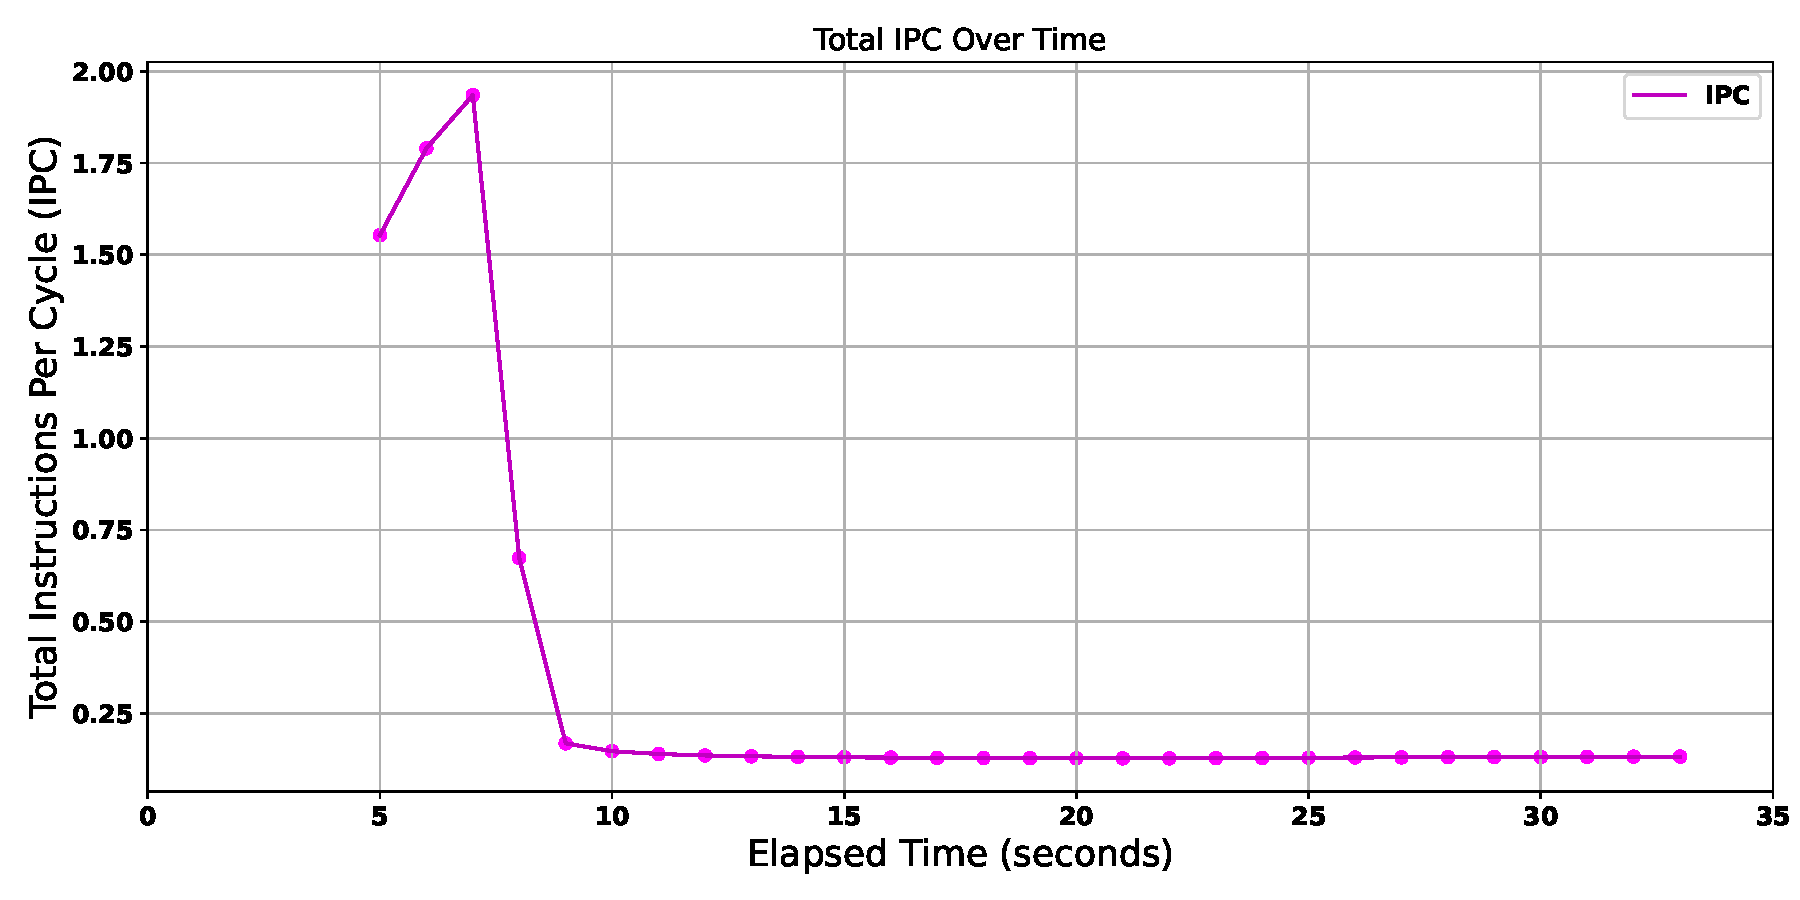
\includegraphics[width=\textwidth]{Figures/IPC_plot.pdf}
%         \caption{$IPC$}
%         \label{fig:IPC}
%     \end{subfigure}\hfill
%     \begin{subfigure}[b]{0.5\textwidth}
%         \centering
%         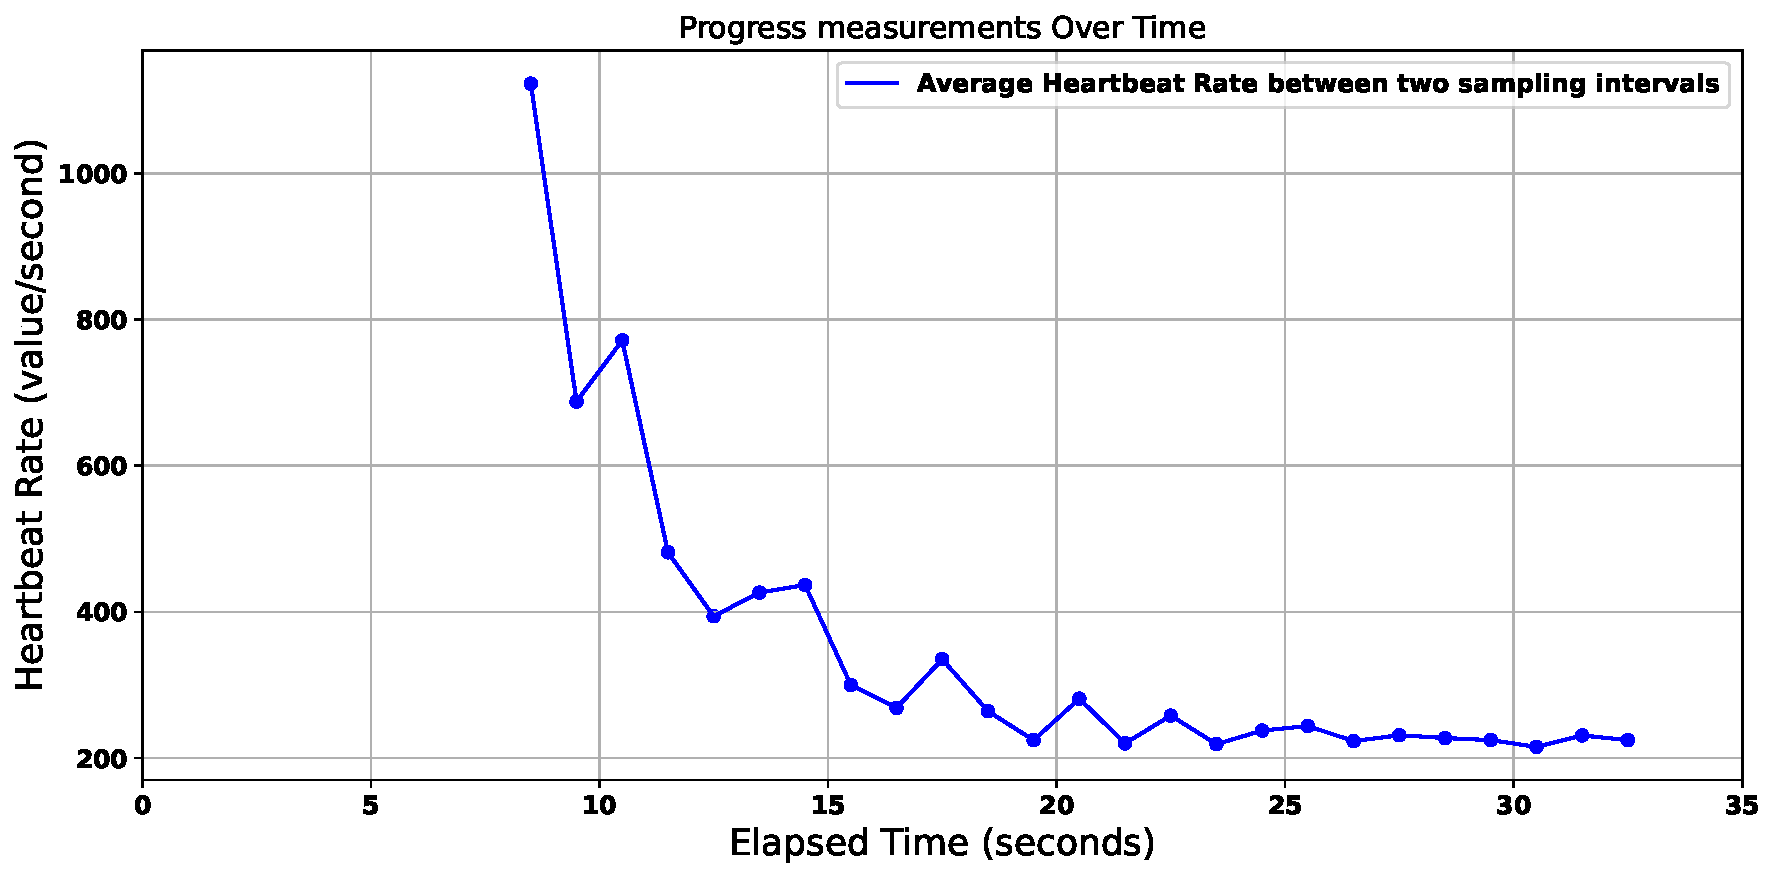
\includegraphics[width=\textwidth]{Figures/progress.pdf}
%         \caption{$Progress$}
%         \label{fig:progress}
%     \end{subfigure}
%     \caption{Comparison of $IPC$ and $progress$ during the runtime of an application (XS-Bench) with progress values displaying more performance granularity.}
%     \label{fig:perf_granularity}
%     \Description{Motivating example}
% \end{figure*}
% \vspace{-0.1cm}

\subsection{Comparison with Related Efforts}\label{sec:relwork}

Energy consumption of compute-intensive applications has been the focus of substantial research in different domains of science and technology including semiconductor design, architecture design, and application design. In this section we discuss relevant practices and techniques in the literature to reduce the energy consumption on compute nodes given the hardware architecture and application. 

Power profiling is the conventional and convenient practice to understand the application phases prior to actual usage. For example, Ryan et al.~\cite{8323587} surveyed different methods used in the analysis of an application's runtime profile, where input power consumption changes. The authors classified the power-profiling methods into in-band and out-of-band, based on the approach used to measure the power consumption of a node. 

For instance, the job-wide energy consumption returned during or at the end of an application runtime, measured using external meters, 
% Akhilesh, I am reducing these citations as it is ok not to have a citation for a product
%such as WattsUp!~\cite{hirst2013watts} and WattProf~\cite{rashti2015wattprof}, 
such as WattsUp! and WattProf, 
is considered out-of-band, while the same data collected by analyzing the measurements from device-level integrated measurement sensors is considered in-band. From the perspective of an application during its execution, in-band measurements are more accurate and useful for dynamic power control. 
% Akhilesh, commenting this out as I feel it does not add anything given it is a survey only paper
\iffalse 
A survey conducted by Labasan et al.~\cite{labasan2016energy} explored state-of-the-art monitoring and controlling tools, such as Intel's RAPL, AMD's Application Power Management, IBM's EnergyScale, and the NVIDIA Management Library.
\fi

Simmendinger et al.~\cite{10740868} highlighted the importance of dynamic power
capping. They showed that adjusting the power available dynamically can allow a management policy to deal with changes in applications' behaviors and also to redistribute
available power to other nodes or resources within a datacenter. 

% Several works have explored system software capable of node-level energy
% optimization. Most notably, the Energy Aware Runtime (EAR)~\cite{corbalan2019ear} is a software solution deployed in production systems capable
% of regulating power at runtime using a model that detects MPI calls (phases) and
% adjusts power caps accordingly. The Dynamic Energy-Performance Optimizer \cite{KRZYWANIAK2023396} takes care of GPU power control by using profiling tools to suggest power across the node. The dynamic power capping algorithm detects phase changes that were observed during
% profiling runs, while it continues with static $PCAP$s for unobserved behaviors.
% Similarly, the Bull Dynamic Power Optimizer \cite{8514915} uses instructions per
% cycle (IPC) to dynamically adjust the core frequencies.

Several works have explored system software for node-level energy optimization. The Energy Aware Runtime (EAR)~\cite{corbalan2019ear} regulates power at runtime using phase detection based on MPI activity, while the Bull Dynamic Power Optimizer~\cite{8514915} rely on profiling and instruction-per-cycles heuristics for control.

In contrast, our approach overcomes the application- and hardware-specific nature of these controllers by being amenable to control of unknown applications, while gathering application-agnostic performance data (heartbeats) for increased adaptability.

% An example of a hybrid hardware-software approach is Performance under Power Limits (PUPiL) ~\cite{zhang2016maximizing}, which manipulates DVFS, core allocation, socket usage, memory usage, and hyperthreading to achieve energy and power consumption benefits. PUPiL was compared to raw RAPL power capping, and the results favored PUPiL. Score-P ~\cite{czarnul2019energy}, designed for analysis and optimization of HPC applications, enables energy-aware analysis and distinguishes between energy-optimal and time-optimal configurations.
% Energy and power management tools use various features of the modern day processors to achieve regulation.
% For instance, Dynamic Voltage and Frequency Scaling (DVFS), discussed in the paper by Gr et. al.~\cite{ge2013effects}, demonstrates its efficiency in CPU and GPU power control by controlling the core and uncore frequencies based on the demand. Another technique, Dynamic Concurrency Throttling (DCT) and concurrency packing ~\cite{czarnul2019energy}, can lead to energy and power savings. However, these methods require an algorithm running in the background to monitor and thereafter take control measures. Therefore adding a measurement and control algorithm to regulate the input given to the DCT adds more workload to the system.

% Some of these above methods provide data related to the ongoing performance of the application and the characteristics which have been extensively used for power regulation and thereby reduce the energy consumption. Such methods along with application phase detectors have been successful in literature to identify the performance bottlenecks and control power using a static power cap throughout the runtime or using automated Dynamic Voltage and Frequency Scaling (DVFS). But phase detectors need a detection threshold which is user defined and varies from application to application. Therefore an observe and control mechanism incorporating both the phase detection and control into a single model, will have a far reaching impact than cascading the models. 

% \textcolor{red}{One approach that computing centers have used to control power consumption is to set a cap on the amount of power a supercomputer uses. Because a supercomputer’s power consumption is determined by the number of processors in the system and the processors’ speed, a “static” approach to power capping can mean throttling processor speed so that the system runs slower than its full capabilities. Although this method can effectively reduce the absolute amount of power consumed, it can negatively affect the performance and throughput of application codes. In a sense, static power capping can reduce the ability of supercomputers to fulfill their key mission: running massively parallel simulations as fast as possible.}


% The work by Cai et.al~\cite{6121386}, classifies energy-aware computing approaches for servers, clusters, data centers, and grids and clouds. However, it does not thoroughly address all the current optimization criteria that exploits the mechanisms for power capping with comprehensive analysis of applications and benchmarks in the field. 
% Our work focuses on the expendable total energy for running workloads with user-defined problem sizes. The proposed RL-algorithm attempts to maintain the run-time energy consumption within the proposed limit.

% %
% In this paper, we aim to automate this control process by utilizing an RL-agent to observe system performance changes using measurements and propose appropriate control actions.

% Therefore, it is crucial to have a power monitoring and controlling tool that can accommodate the proposed control algorithm between its sensors and actuators. 


% Followingly, Desrochers et al. ~\cite{desrochers2016validation} validated the CPU RAPL measurement accuracy by using RAPL DRAM power measurements with different DDR3 and DDR4 memory types, and comparing them with readings from an actual hardware power meter. Intel's RAPL, therefore, is an indispensable tool for power monitoring and control algorithms in the field of energy-efficient computing. In our work we leverage the capabilities of Intel RAPL which forms an essential tool for monitoring and controlling power/energy consumption in our proposed control algorithm that utilizes an RL-agent for automated control in energy management irrespective of the benchmark application it runs. 
% Similarly, Raghavendra et al. ~\cite{raghavendra2008no} implemented a controller that stops power supply to subsystems by detecting no-load zones during application execution, enabling fine-grained power regulation. However, the efficiency of workload characteristic detection in their hardware-centric approach is not optimal, as the focus of the research primarily lies in the hardware aspects.
In another study, Cerf et al.~\cite{cerf2021sustaining} used a control theoretical approach  to attenuate disturbances in performance under reduced power supply. They designed a classical proportional-integral-derivative controller to impose power caps on RAPL actuators using performance feedback from the compute nodes. The controller was shown to track a user-defined performance set point.

%The use of ML techniques that can simultaneously optimize performance and power is on the rise. Such methods 
More recently, ML techniques have demonstrated increased efficacy in managing online job scheduling and hardware configurations \cite{chen2015distributed,10571824}, offering broad applicability across various applications, where modeling the relationship between cluster node configurations and performance is impractical.

Prior efforts using RL in the control of compute node energy efficiency exist. Wang et al.~\cite{10.1145/3716872} proposed an online power control algorithm by observing the total instructions per cycle ($IPC$)  while running an application and thereby regulating core and uncore frequencies with online interactions during the execution of applications to enhance learning. However, Ramesh et al. \cite{ramesh2019understanding} show that $IPC$ is an unsuitable performance metric for compute-intensive applications as it fails to distinguish useful application progress from idle-time activity, both of which contribute to the total instruction count. 

Likewise, the authors in~\cite{10305814} used RL trained on a mathematical model of a modified STREAM benchmark to regulate power of HPC nodes through RAPL actuators. But the process of generating a mathematical model for each  application's behavior to be trained is cumbersome. 

In relation to these works,  we formally introduce an offline RL-based dynamic power management algorithm that is independent of phase detectors and surrogate models and is capable of managing power across diverse hardware and applications to ensure optimal energy utilization at runtime.
% \vspace{-0.5cm}
% The choice of power optimization method often depends on the specific hardware being used. For instance, Caglar et al.~\cite{caglar2014iplace} explored software-based approaches for power optimization, employing duty cycle, voltage, and frequency scaling. Their work utilized machine learning techniques to model application performance and hardware characteristics, enabling informed placement decisions. However, software-based algorithms, such as the one proposed by  Jung et al. \cite{jung2010supervised}, which utilizes supervised learning for power management in multi-core processors, is not always be reliable due to the need for extensive training data prior to implementation.


% {In the paper the authors were able to excite the HPC node running the STREAM benchmark at all the regions of operation. But the variations in the mathematical model with the benchmark application it runs made the proposal for a generalized controller difficult.} 

% Considering the limitations of ~\cite{cerf2021sustaining}, we emphasize the design of an optimal controller to solve the underlying power and performance optimization problem. Our proposed approach takes a hybrid stance, utilizing instantaneous performance analysis obtained through state-of-the-art algorithms to determine the best operating power cap for compute nodes.